\documentclass{article}

% if you need to pass options to natbib, use, e.g.:
% before loading neurips_2023


% ready for submission
%\usepackage{neurips_2023}


% to compile a preprint version, e.g., for submission to arXiv, add add the
% [preprint] option:
%     \usepackage[preprint]{neurips_2023}


% to compile a camera-ready version, add the [final] option, e.g.:
\usepackage[final]{neurips_2023}


% to avoid loading the natbib package, add option nonatbib:
%    \usepackage[nonatbib]{neurips_2023}


\usepackage[utf8]{inputenc} % allow utf-8 input
\usepackage[T1]{fontenc}    % use 8-bit T1 fonts
\usepackage{hyperref}       % hyperlinks
\usepackage{url}            % simple URL typesetting
\usepackage{booktabs}       % professional-quality tables
\usepackage{amsfonts}       % blackboard math symbols
\usepackage{nicefrac}       % compact symbols for 1/2, etc.
\usepackage{microtype}      % microtypography
\usepackage{xcolor}         % colors
\usepackage{caption}
\usepackage{subcaption}
\usepackage{amsmath, amsfonts, mathtools, amsthm, amssymb}
\usepackage{mathrsfs}

\usepackage[utf8]{inputenc}
\usepackage[T1]{fontenc}
\usepackage{textcomp}
% \usepackage[dutch]{babel}
\usepackage{url}
% \usepackage{hyperref}
% \hypersetup{
%     colorlinks,
%     linkcolor={black},
%     citecolor={black},
%     urlcolor={blue!80!black}
% }
\usepackage{graphicx}
\usepackage{float}
\usepackage{booktabs}
\usepackage{enumitem}
% \usepackage{parskip}
\usepackage{emptypage}
\usepackage{subcaption}

\title{Cloth Simulation with Character Collisions}


\author{%
  Patrick Tourniaire \\
  École Polytechnique \\
  \texttt{patrick.tourniaire@polytechnique.edu}
}


\begin{document}


\maketitle


\begin{abstract}
  \textit{To be completed}
\end{abstract}


\section{Introduction}


\section{Notation}

Throughout this report we will be referring to vectors in a 3D scene in bold (such as $\mathbf{x}$), and 
scalar values unbolded (such as $r$ for radius).

\section{Methodology}

To be able to construct an effective approach to dealing with cloth collisions with a character
whilst keeping the complexity at a reasonable level, we make a few simplifying assumptions. Dealing
with collisions with primitive shapes such as spheres and cylinders is much more trivial than dealing with
the endless edg-cases when using a high detail character mesh. Thus, for our character we use a skeleton
and set joints to be spheres and have cylinders represent the connections between joints. Thus enabling
us to take this simpler approach whilst still achieving the goal. 

\subsection{From Skeleton to a Character of Primitive Shapes}

The character we will be dealing with is the Lola character from previous works. This character obviously
have a much higher complexity than a skeleton built of primitive shapes. Thus, we optimise the radius of
the spheres and cylinders such that they only slightly cover the mesh surface, an example of these primitive
shapes on the skeleton can be observed in Figure \ref{fig:methodology/skeleton}. As we will observe in Section
\ref{sec:/results}. 

\begin{figure}[!ht]
  \centering
  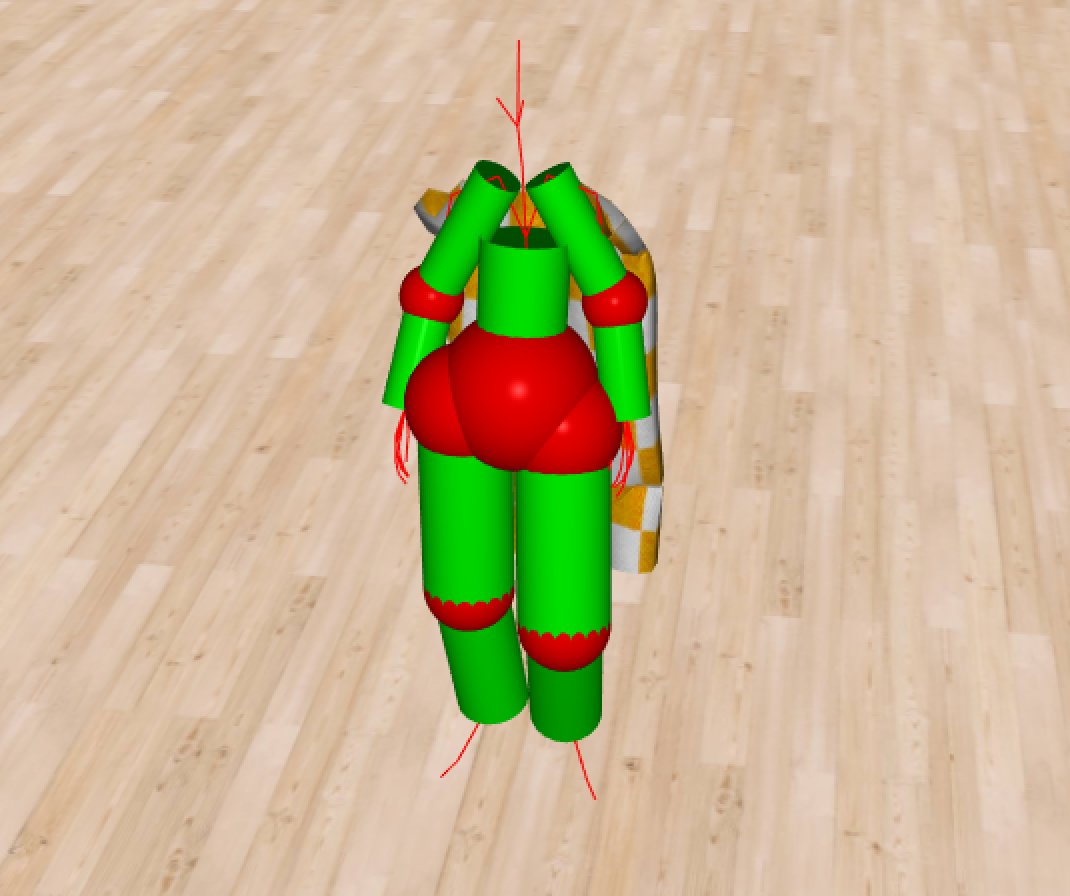
\includegraphics[width=.4\linewidth]{figs/skeleton.png}
  \caption{Showing how we construct a simple mesh for collision detection using primitive shapes such as spheres
  and cylinders exclusively Note how only a few essential bone segments have primitive collision shapes as most
  bone segments would be redundant to deal with collisions.}
  \label{fig:methodology/skeleton}
\end{figure}

\subsection{Collision with Primitive Shapes}

In this section we will be presenting the different forms of constraints which our system deals with to
avoid collisions between the cape and the character. As we aim to simulate a cape on the character, a natural
question to ask is; how do we fix the cape to the character whilst it is moving? 

We can frame this as a constraint in our system, however, it is not a collision constraint in this case.
It is simply enforced through 4 points on the cape which should always have the same position as some points/joints on
the skeleton. We have decided to use 4 attach points due to the fact that 2 attach points can lead to the
cape being elongated significantly whilst the character is moving. Thus, the first attach point is located on
the left shoulder, the second on the midpoint between the left shoulder and the upper spine, the third is located 
on the midpoint between the upper spine and the right shoulder, and finally the fourth point is attached to the
right shoulder. As we will observe in Section \ref{sec:/results} this achieved much better results than only using
shoulders as attach points.


\subsubsection{Planes}

Dealing with collisions with planes is trivial, however, it will serve as a good foundation for how we deal with
sphere and cylindrical constraints. Assume we have some plane parametrised by a normal vector $\mathbf{n}_{\text{ground}}$.
Then, we simply check that if the y-component of some cape particle is below the y-component of the normal. If that is the
case then we perform the following update, where $\mathbf{p}_i$ represents some ith particle in the cape.

\begin{align}
  \mathbf{p}^{(y)}_i = \mathbf{n}^{(y)}_{\text{ground}} + \epsilon
\end{align}

Where $\epsilon$ represents some offset from the ground, which is set based on the physical thickness of the cape.

\subsubsection{Spheres}

To deal with sphere collisions, we take the following approach. First, every particle making up the mesh
of the cloth will be compared with every single joint which has a spherical constraint. We note that not
all joints have spherical constraints as this would be redundant for a multitude of smaller joints (such as
finger joints). Let us denote some particle $\mathbf{p}$ to be a particle in the cape, and some sphere center
by $\mathbf{c}$ with some radius $r$. We can detect a collision by evaluating the following distance.

\begin{align}
  ||\mathbf{c} - \mathbf{p}|| \leq r + \epsilon
\end{align}

Here we introduce some $\epsilon$ such that we do not place the cape particle on the edge of the sphere.
For our case, we set this to be a small enough value to reflect the thickness of the fabric, such that the
cape does not slightly penetrate the surface of the joint sphere. The update step for the new position of
the cape particle becomes.

\begin{align}
  \mathbf{p}' = (r + \epsilon) \mathbf{n}
\end{align}

Where $\mathbf{n}$ represents the unit normal, obtained by normalising $(\mathbf{p} - \mathbf{c})$.

\subsubsection{Cylinders}

The approach for dealing with cylindrical constraints is quite similar to the one presented for spheres. 
However, there is an additional layer of complexity added. We parametrise a cylinder by the following, it
starts at some joint $\mathbf{p}_i$ and ends at some other joint $\mathbf{p}_j$, with some constant radius
of $r$. Thus, we only want to define a collision when a cape particle is within this bone segment and is
within the radius plus some additional $\epsilon$. We determine this by projecting every cape particle on
the bone segment spanning the cylinder and checking if the following two conditions hold. First we define
the projection by the following.

\begin{align}
  \mathbf{p}_{\text{proj}} = \dfrac{\mathbf{p} (\mathbf{p}_i - \mathbf{p}_j)}{||\mathbf{p}_i - \mathbf{p}_j||}
\end{align}

Then evaluate the following conjunct to determine if we need to check that the particle is within the radius
of the cylinder or not.

\begin{align}
  || p_{\text{proj}} - \mathbf{p}_i || \leq ||\mathbf{p}_i - \mathbf{p}_j||  \hspace{2.5mm}  \bigwedge \hspace{2.5mm} || \mathbf{p}_{\text{proj}} - \mathbf{p}_j ||  \leq ||\mathbf{p}_i - \mathbf{p}_j|| 
\end{align}

If this conjunct returns true, then we will evaluate if the particle is within the bounds of the mesh surface or
not. Which is achieved by evaluating the following inequality.

\begin{align}
  || \mathbf{p} - \mathbf{p}_{\text{proj}} || \leq r + \epsilon
\end{align}

If this condition is true then we perform the following update step for the cape particle. Where $\mathbf{n}_{\text{proj}}$
represents the unit normal of $\mathbf{p} - \mathbf{p}_{\text{proj}}$.

\begin{align}
  \mathbf{p}' = (r + \epsilon) \mathbf{n}_{\text{proj}}
\end{align}

Through this approach we are able to use both spheres and cylinders to effectively create a rough framework
for achieving, cloth-character collisions. However, we also apply external forces such as gravity and wind to
the cape to acheive realistic results.

\subsection{Physical Forces}

The physical forces applied to the cape are wind, gravity and spring forces applied between cape particles.
How we have applied this is similar to past works we have done and thus, we will not go into detail. However,
we will present a brief overview for the sake of reproducibility.

\subsubsection{Inter-Particle Spring Forces}

\subsubsection{Gravity}

\subsubsection{Wind}

\subsection{Complete Algorithm}

\subsection{Character Movement}

The character movement is based on the previous works done, where we have a static animation for walking which
is played in a loop. Then to achieve a seamless transition from animation start to animation end we perform a
quaternion interpolation of each local joint frame of the skeleton from the end state to the start state.
Thus, when the character stops moving a transition starts from the walking state to the idle state to also 
achieve this seamless transition between states.


\section{Qualitative Results} \label{sec:/results}

\begin{figure}[ht]
  \centering
  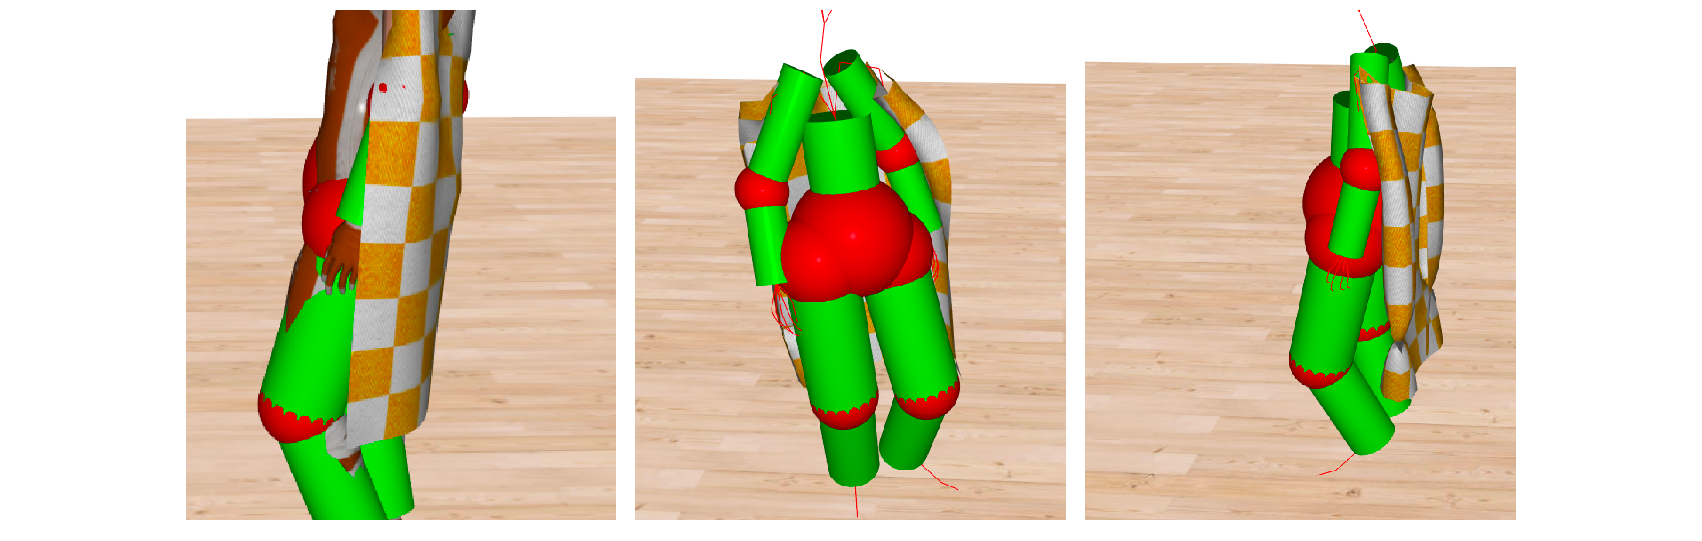
\includegraphics[width=\linewidth]{figs/qualitative_results.pdf}
  \caption{Qualitative results achieved for cloth collision with primitive shapes making up the character skeleton.
  Left image shows how these primitive shapes overlap slightly the complex mesh for the character.}
  \label{fig:results/results}
\end{figure}

Based on the results observed in Figure \ref{fig:results/results} we achieve decent approximations for the
collisions with the complex mesh of the character. We note that the framerates do not drop after adding these
constraints with the primitive shapes given that our approach is not computationally heavy. However, there are
quite a few limitations with our approach.

If one looks more closely at smaller bone sgements such as fingers there are cases where they can poke through
the cape, however, one would have to look very carefully to notice. We can go around this by simply adding constraints
on the fingers using very small cylinders. However, that will not solve the issue by itself as the character can move
quite fast wrt to the numerical approximation of the particle forces. Thus, in most cases the cape would be able to
teleport through these shapes before our approach would be able to detect a collision and thus perform the iterative
updates to the forces applied to the cape particles. One could in theory decrease the time delta for this approaximation
but one would have to set an extremely low time delta which would result in unstable results. Another naive approach
would be to slow down the movement of the character however this does not resolve the issue directly.

Therefore, this discussion highlights the downside of approximation methods for the computation of forces. To achieve
better results one could apply more complex and exact techniques such as FastMassSpring presented by Tiantian Liu, et al.
\cite{FastMassSpring}.



\section{Conclusion}


\section*{References}


{
  \small
  \bibliographystyle{plain} % We choose the "plain" reference style
  \bibliography{refs} % Entries are in the refs.bib file
}

%%%%%%%%%%%%%%%%%%%%%%%%%%%%%%%%%%%%%%%%%%%%%%%%%%%%%%%%%%%%


\end{document}